\begin{table}[H]
\centering\small\tablaestilo
\caption{Resultados de las dos pruebas de falla.}
\label{tab:p2}
\begin{tabularx}{\textwidth}{|>{\raggedright\arraybackslash\bfseries}p{4.1cm}|Y|Y|}
\hline
\encab \hd{Aspecto} & \hd{P2.1 Falla lógica} & \hd{P2.2 Falla abrupta} \\ \hline
Qué hicimos & Un servidor empieza a reportarse como enfermo & Borramos un servidor con usuarios activos \\ \hline
Deja de recibir tráfico & \textbf{a los 8 segundos} & a los 3 segundos (se apaga) \\ \hline
Errores durante la falla & \textbf{1,7\,\%}, igual que antes de la falla & \textbf{29\,\%} solo durante los primeros 15\,s \\ \hline
Cómo se recupera & Azure lo \textbf{reemplaza solo} a los 11 minutos & El autoscale crea otro en \textbf{109 segundos} \\ \hline
\end{tabularx}
\end{table}

\begin{figure}[H]
\centering
\begin{subfigure}{0.49\textwidth}
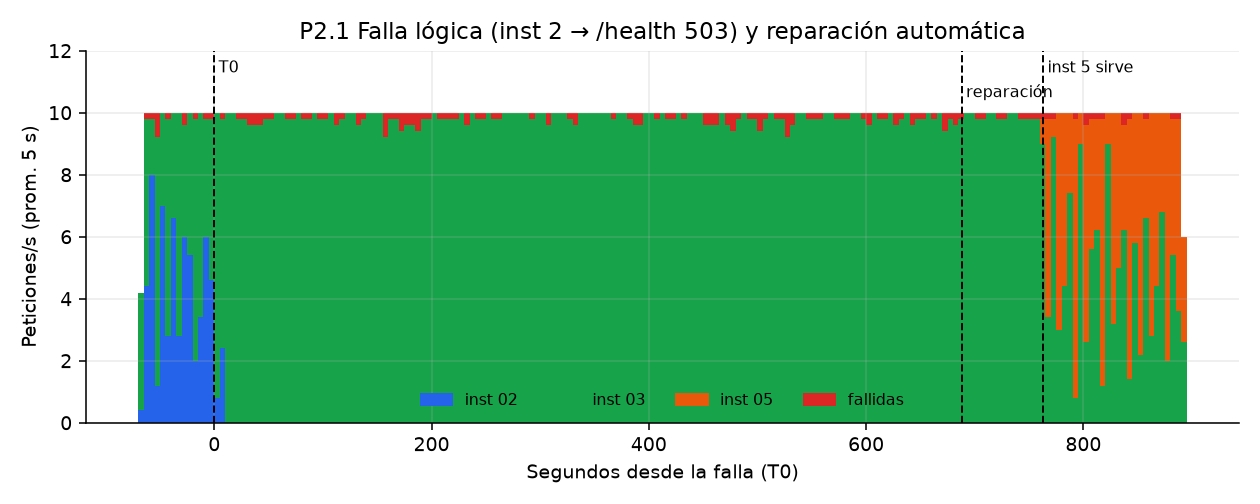
\includegraphics[width=\linewidth]{figuras/p2_logica.png}
\caption{Falla lógica.}
\end{subfigure}\hfill
\begin{subfigure}{0.49\textwidth}
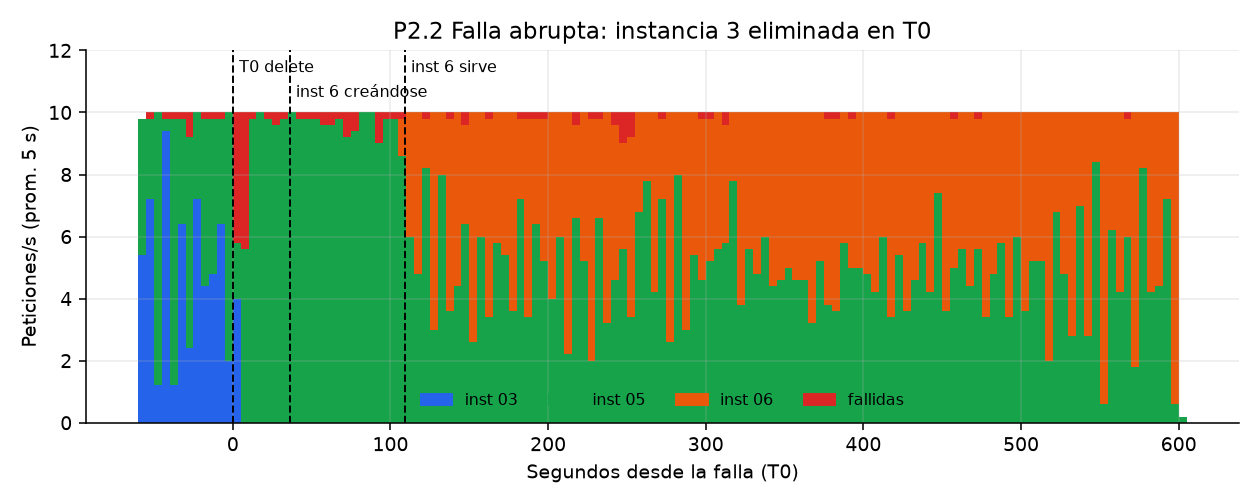
\includegraphics[width=\linewidth]{figuras/p2_abrupta.png}
\caption{Falla abrupta.}
\end{subfigure}
\caption{Peticiones por segundo que atendió cada servidor (colores) y las fallidas (rojo).}
\label{fig:p2}
\end{figure}

\begin{figure}[H]
\centering
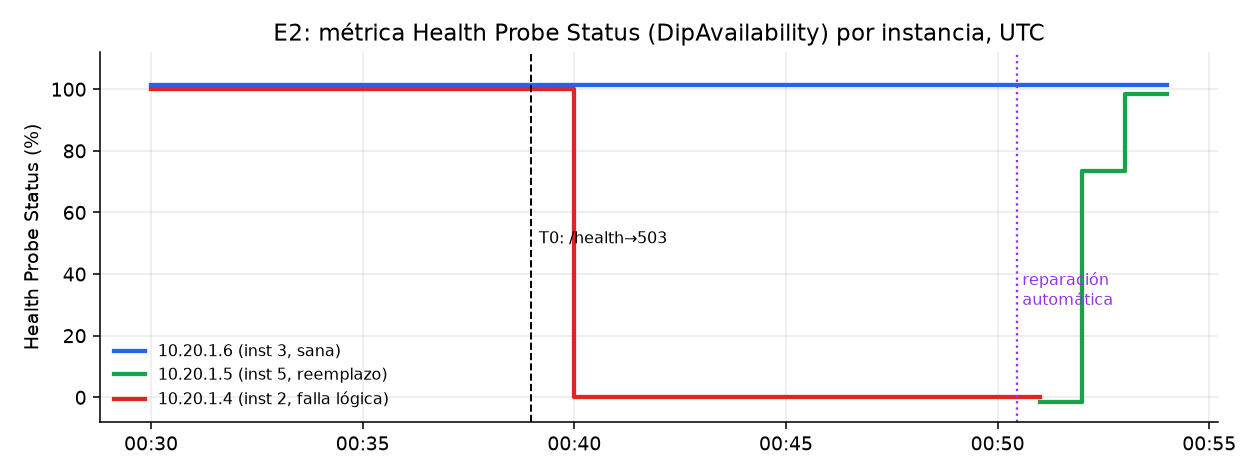
\includegraphics[width=0.6\textwidth]{figuras/e2_health_probe.png}
\caption{Salud de cada servidor según el balanceador: el servidor con falla queda en 0\,\% hasta que lo reemplazan.}
\label{fig:p2logica}
\end{figure}

\textbf{Análisis.} La falla lógica pasó desapercibida para los usuarios: el servidor siguió
respondiendo lo que tenía en curso mientras el balanceador lo retiraba, y el porcentaje de error
no cambió (esos pocos errores vienen de nuestra red doméstica y ya estaban antes de la falla). La
falla abrupta sí se notó, pero solo unos 15 segundos: es lo que tarda el balanceador en confirmar,
con dos revisiones de 5\,s, que el servidor ya no existe. Con más servidores en línea, la parte
afectada del tráfico sería menor. La reparación automática fue lenta (11 minutos) porque Azure
espera 10 minutos antes de reemplazar; el autoscale, en cambio, repuso la capacidad en menos de
2 minutos.
